
\section{Ellipsoids}

%%%%%%%%%%%%%%%%%%%%%%%%%%%%%%%%%%%%%%%%%%%%%%%%%%%%%%%%%%%%%%%%%%%%%%%%%%%%%%%%
%%%                        SUBSECTION: INTRODUCTIONS                         %%%
%%%%%%%%%%%%%%%%%%%%%%%%%%%%%%%%%%%%%%%%%%%%%%%%%%%%%%%%%%%%%%%%%%%%%%%%%%%%%%%%

\subsection{Definitions}
Our first motivating question is \textbf{``what is an ellipsoid?''}
We are all familiar with the definition of an ellipse from
calculus, namely the set of points satisfying
%
\begin{equation}\label{eq:naive-ellipse}
  \left(\frac xc\right)^2 + \left(\frac yd\right)^2 \leq 1.
\end{equation}
%
This form, of course, does not completely characterize all ellipses since we
need to handle rotations and translations, but it's enough to get us started. We
turn these constraints into matrix form:
%
\begin{equation}\label{eq:naive-ellipse-matrix}
  \left(\begin{matrix}x&y\end{matrix}\right)
  \left(\begin{matrix}c^{-2} &0\\0&d^{-2}\end{matrix}\right)
    \left(\begin{matrix}x\\t\end{matrix}\right)\leq 1
\end{equation}
%
This matrix is positive definite, and we can genearlize the definition of an
ellipse to that of an ellipsoid:

\begin{defbox} 
  \begin{definition}[ellipsoid, \(E(A, a)\)]

    For positive definite \(n\times n\) matrix \(A\), the set of points
    %
    \begin{equation}\label{eq:def-ellipsoid}
      E(A,a) = \{x \in \R^n : (x - a)^T A^{-1} (x - a) \leq 1\}
    \end{equation}
    %
    is called an \textbf{ellipsoid}.\footnote{Some sources define an ellipsoid
    to be the boundary \(\partial E\) by setting the inequality in
    (\ref{eq:def-ellipsoid}) to be equality. For our purposes our current
    definition is more useful.}
    Vector \(a\) is called the \textbf{center}
    of \(E(A, a)\), and \(E(A,a)\) is referred to as \textbf{the ellipsoid
    associated with \(A\) and \(a\)}.\qed
  \end{definition}
\end{defbox}

\begin{examplebox}{An ellipse is an ellipsoid}
  \begin{example}
    The ellipse \(E\) in (\ref{eq:naive-ellipse}) may be put into matrix form
    in (\ref{eq:naive-ellipse-matrix}). Taking
    %
    \[A^{-1} = \left(\begin{matrix} c^{-2} & 0\\ 0 & d^{-2} \end{matrix}\right)\]
    %
    we compute
    %
    \[A = \left(\begin{matrix} c^2 & 0\\ 0 & d^{2} \end{matrix}\right)\]
    %
    and we can write
    \[E = E(A, 0).\]
  \end{example}
\end{examplebox}

Unless it changes a calculation we will assume all ellipsoids are centered at
the origin, making the algebra easier,  but unless otherwise stated, all results
proved for ellipsoids centered at the origin hold for arbitrary ellipsoids.

%%%%%%%%%%%%%%%%%%%%%%%%%%%%%%%%%%%%%%%%%%%%%%%%%%%%%%%%%%%%%%%%%%%%%%%%%%%%%%%%
%%%               SUBSECTION: RELATING ELLIPSOIDS AND SPHERES                %%%
%%%%%%%%%%%%%%%%%%%%%%%%%%%%%%%%%%%%%%%%%%%%%%%%%%%%%%%%%%%%%%%%%%%%%%%%%%%%%%%%

\subsection{Relating Ellipsoids and Spheres}
Here we make precise the notion of shmooshing.
The unit ball centered at \(a\) is a special case of the ellipsoid
\(\ball(1, a) = E(I, a),\) since
%
\[\ball(1, a)  = \{x : (x - a)^T(x - a) < 1\} = \{x : (x - a)^T I (x - a) \leq 1\} = E(I, a)\]
%
It turns out we can also write ellipsoids \(E(A, a)\) as affine transformation
of \(\ball(1,0)\), namely
%
\[E(A,a) = A^{1/2} \ball(1, 0) + a.\]
%
Here \(A^{1/2}\) is the unique positive definite matrix satisfying
\[A = A^{1/2} \cdot A^{1/2},\]
whose existence is a well-known property of positive definite matrices.\\

\begin{figure}[t]
  \centering
  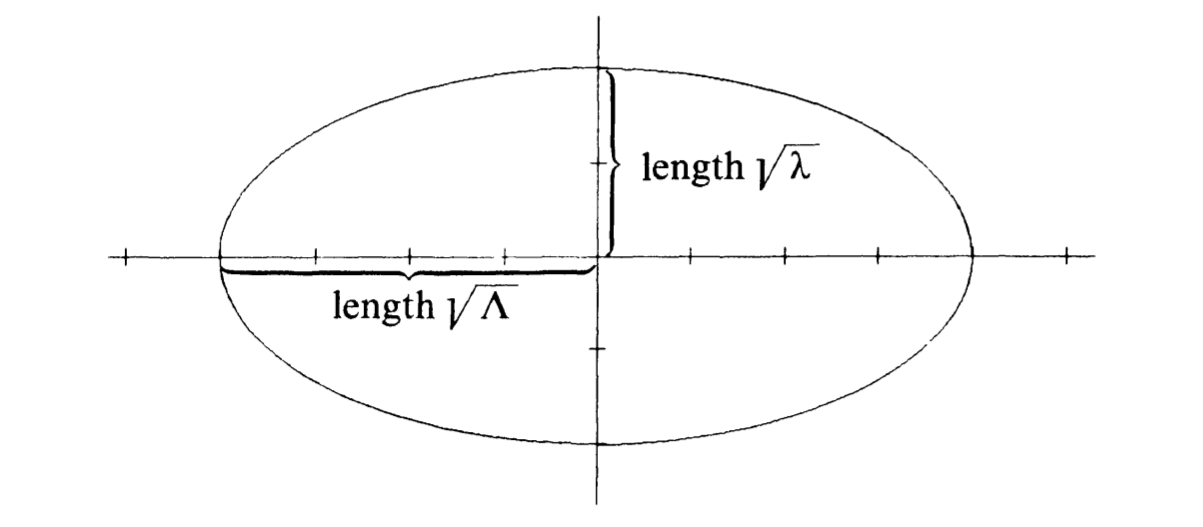
\includegraphics[width=0.75\textwidth]{img/ellipsoid}
  \caption{An ellipsoid}
  \label{fig:ellipsoid-eigenvalue}
\end{figure}
\begin{examplebox}{\textbf{Example of an ellipsoid in \(R^2\):} \textit{ellipsoids and
  eigenvalues}}
  \begin{example} Consider the ellipsoid in
    Figure~\ref{fig:ellipsoid-eigenvalue}. This ellipsoid may be written in the
    form \(E(A,0)\), where
    \[A = \left(\begin{matrix}
      \Lambda & 0\\
      0 & \lambda
    \end{matrix}\right),\]
    where \(\lambda < \Lambda\) are the two eigenvalues of \(A\).
  \end{example}
\end{examplebox}

\begin{fact}
  The volume of \(E(A,a)\) can be calculated as
  %
  \[\vol(E(A, a)) = \sqrt{\det A} \cdot V_n,\]
  %
  where \(V_n\) is the volume of the unit ball \(\ball_n(1,0)\), where we
  subscript by \(n\) to make explicit the balls dimension. While explicit
  formulas are known, for our purposes it suffices to know that
  %
  \[n^{-n} \leq V_n \leq 2^n.\]
  %
  What's more, given an affine transformation \(T\) preserves the quotient of
  the volumes of ellipsoids \(E_1\) and \(E_2\)
  %
  \[\frac{\vol(E_1)}{\vol(E_2)} = \frac{\vol(T(E_1))}{\vol(T(E_2))}.\]
  %
  \todo{This should be given later closer to where we need it, otherwise our
  audience will forget all about it}
\end{fact}

